% Asynchronous execution, kept simple: R calls a jitted function twice, runs other code, and only
% then needs the values. The code, and a timeline of R and the device (not to scale), with the
% device's work in the accent color and R's waiting in gray. Shared style in style.tex.
% Build: make figures/async.pdf
\documentclass[tikz, border = 6pt]{standalone}
% The style shared by the TikZ figures of the paper (overview.tex, tracing.tex, async.tex):
% fonts, the colors of the packages, the highlight color, and the styles of boxes, headings,
% numbered badges, and notes. benchmarks/plots.R uses the same colors and font for the plots.
\usepackage[T1]{fontenc}
\usepackage{lmodern}
\usetikzlibrary{positioning, calc, fit, backgrounds, matrix, arrows.meta}

% Colors of the packages, as in the overview figure (after the mlr3torch figures).
\definecolor{tealframe}{HTML}{21908c}
\definecolor{lightbox}{HTML}{e4f1f1}
\definecolor{viridis1}{HTML}{8e6698}
\definecolor{viridis8}{HTML}{ccea84}
\definecolor{modelgrey}{HTML}{e5e5e5}
\colorlet{cr}{white}
\colorlet{canvl}{lightbox}
\colorlet{cstablehlo}{viridis1!22}
\colorlet{cpjrt}{viridis8!45}
\colorlet{cquickr}{modelgrey}

% The highlight color: the part of a figure that shows its point.
\colorlet{accent}{tealframe}

\newcommand{\cd}[1]{\texttt{#1}}
\newcommand{\hl}[1]{\textcolor{accent}{#1}}

\tikzset{
  % a box around a part of a figure, and its heading
  box/.style = {rounded corners = 2pt, inner sep = 5pt},
  plainbox/.style = {box, draw = black!25, fill = black!4},
  framebox/.style = {box, draw = black!40},
  accentbox/.style = {box, draw = accent!80!black, fill = accent!7},
  head/.style = {font = \footnotesize\bfseries, text = black!70, anchor = south west,
    inner sep = 1pt},
  % a number that links a part of a figure to a note
  badge/.style = {circle, fill = black!65, text = white, font = \sffamily\tiny\bfseries,
    inner sep = 0pt, minimum size = 3.2mm, anchor = base},
  note/.style = {font = \footnotesize, align = left, text width = 7.4cm, anchor = north west,
    inner sep = 0pt, execute at begin node = {\thickmuskip = 5mu}},
  % lines of code or of a printed graph, followed by columns of badges
  lines/.style = {matrix of nodes, row sep = {3.9mm, between origins}, column sep = 2pt,
    nodes = {anchor = base west, inner sep = 0.5pt, font = \ttfamily\scriptsize}},
  % rows of a name and its value(s)
  fields/.style = {matrix of nodes, row sep = {3.9mm, between origins}, column sep = 2pt,
    nodes = {anchor = base west, inner sep = 0.5pt, font = \ttfamily\scriptsize},
    column 1/.style = {nodes = {text = black!55}}},
  flow/.style = {-{Stealth[length = 1.6mm]}, black!55, thin}
}

% A note: its text at #2, numbered #1 in a badge hanging to its left.
\newcommand{\note}[3]{
  \node[note] (#1) at #2 {#3};
  \node[badge, font = \sffamily\scriptsize\bfseries, minimum size = 3.8mm, anchor = north east]
    at ($(#1.north west) + (-0.15, 0.04)$) {#1};
}


\tikzset{
  code/.style = {lines, column 2/.style = {nodes = {text = black!45}}},
  lane/.style = {font = \footnotesize, text = black!70, anchor = east},
  span/.style = {draw, rounded corners = 1pt, minimum height = 5mm, inner sep = 1pt,
    font = \ttfamily\scriptsize, anchor = west},
  rwork/.style = {span, draw = black!45, fill = black!8},
  rwait/.style = {span, draw = black!35, dashed, fill = white, text = black!45},
  dwork/.style = {span, draw = accent!80!black, fill = accent!15, text = accent!60!black}
}

\begin{document}
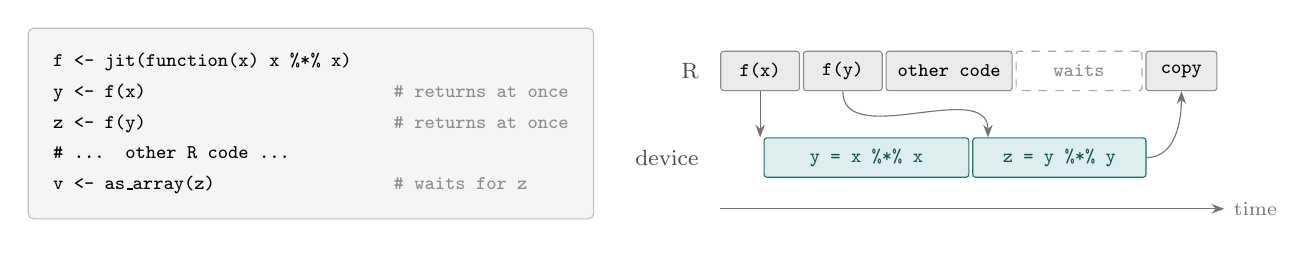
\begin{tikzpicture}

  \matrix[code] (code) at (0, 0) {
    f <- jit(function(x) x \%*\% x) &[12pt] \\
    y <- f(x) & \# returns at once \\
    z <- f(y) & \# returns at once \\
    \# ... other R code ... & \\
    v <- as\_array(z) & \# waits for z \\
  };
  \begin{scope}[on background layer]
    \node[plainbox, fit = (code)] (codebox) {};
  \end{scope}

  % The timeline, not to scale: R on top, the device below.
  \begin{scope}[shift = {($(codebox.north east) + (1.6, -0.55)$)}]
    \node[lane] at (-0.15, 0) {R};
    \node[lane] at (-0.15, -1.1) {device};

    \node[rwork, minimum width = 1.0cm] (call1) at (0, 0) {f(x)};
    \node[rwork, minimum width = 1.0cm] (call2) at (1.05, 0) {f(y)};
    \node[rwork, minimum width = 1.6cm] (other) at (2.1, 0) {other code};
    \node[rwait, minimum width = 1.6cm] (wait) at (3.75, 0) {waits};
    \node[rwork, minimum width = 0.9cm] (copy) at (5.4, 0) {copy};

    \node[dwork, minimum width = 2.6cm] (dy) at (0.55, -1.1) {y = x \%*\% x};
    \node[dwork, minimum width = 2.2cm] (dz) at (3.2, -1.1) {z = y \%*\% y};

    \draw[flow] (call1.south) -- (call1.south |- dy.north);
    \draw[flow] (call2.south) to[out = -90, in = 90] ($(dz.north west) + (0.2, 0)$);
    \draw[flow] (dz.east) to[out = 0, in = -90] (copy.south);
    \draw[flow] (0, -1.75) -- (6.4, -1.75) node[right, font = \scriptsize, text = black!55] {time};
  \end{scope}

\end{tikzpicture}
\end{document}
